% Options for packages loaded elsewhere
\PassOptionsToPackage{unicode}{hyperref}
\PassOptionsToPackage{hyphens}{url}
\PassOptionsToPackage{dvipsnames,svgnames,x11names}{xcolor}
%
\documentclass[
  letterpaper,
  DIV=11,
  numbers=noendperiod]{scrartcl}

\usepackage{amsmath,amssymb}
\usepackage{iftex}
\ifPDFTeX
  \usepackage[T1]{fontenc}
  \usepackage[utf8]{inputenc}
  \usepackage{textcomp} % provide euro and other symbols
\else % if luatex or xetex
  \usepackage{unicode-math}
  \defaultfontfeatures{Scale=MatchLowercase}
  \defaultfontfeatures[\rmfamily]{Ligatures=TeX,Scale=1}
\fi
\usepackage{lmodern}
\ifPDFTeX\else  
    % xetex/luatex font selection
\fi
% Use upquote if available, for straight quotes in verbatim environments
\IfFileExists{upquote.sty}{\usepackage{upquote}}{}
\IfFileExists{microtype.sty}{% use microtype if available
  \usepackage[]{microtype}
  \UseMicrotypeSet[protrusion]{basicmath} % disable protrusion for tt fonts
}{}
\makeatletter
\@ifundefined{KOMAClassName}{% if non-KOMA class
  \IfFileExists{parskip.sty}{%
    \usepackage{parskip}
  }{% else
    \setlength{\parindent}{0pt}
    \setlength{\parskip}{6pt plus 2pt minus 1pt}}
}{% if KOMA class
  \KOMAoptions{parskip=half}}
\makeatother
\usepackage{xcolor}
\setlength{\emergencystretch}{3em} % prevent overfull lines
\setcounter{secnumdepth}{-\maxdimen} % remove section numbering
% Make \paragraph and \subparagraph free-standing
\makeatletter
\ifx\paragraph\undefined\else
  \let\oldparagraph\paragraph
  \renewcommand{\paragraph}{
    \@ifstar
      \xxxParagraphStar
      \xxxParagraphNoStar
  }
  \newcommand{\xxxParagraphStar}[1]{\oldparagraph*{#1}\mbox{}}
  \newcommand{\xxxParagraphNoStar}[1]{\oldparagraph{#1}\mbox{}}
\fi
\ifx\subparagraph\undefined\else
  \let\oldsubparagraph\subparagraph
  \renewcommand{\subparagraph}{
    \@ifstar
      \xxxSubParagraphStar
      \xxxSubParagraphNoStar
  }
  \newcommand{\xxxSubParagraphStar}[1]{\oldsubparagraph*{#1}\mbox{}}
  \newcommand{\xxxSubParagraphNoStar}[1]{\oldsubparagraph{#1}\mbox{}}
\fi
\makeatother


\providecommand{\tightlist}{%
  \setlength{\itemsep}{0pt}\setlength{\parskip}{0pt}}\usepackage{longtable,booktabs,array}
\usepackage{calc} % for calculating minipage widths
% Correct order of tables after \paragraph or \subparagraph
\usepackage{etoolbox}
\makeatletter
\patchcmd\longtable{\par}{\if@noskipsec\mbox{}\fi\par}{}{}
\makeatother
% Allow footnotes in longtable head/foot
\IfFileExists{footnotehyper.sty}{\usepackage{footnotehyper}}{\usepackage{footnote}}
\makesavenoteenv{longtable}
\usepackage{graphicx}
\makeatletter
\def\maxwidth{\ifdim\Gin@nat@width>\linewidth\linewidth\else\Gin@nat@width\fi}
\def\maxheight{\ifdim\Gin@nat@height>\textheight\textheight\else\Gin@nat@height\fi}
\makeatother
% Scale images if necessary, so that they will not overflow the page
% margins by default, and it is still possible to overwrite the defaults
% using explicit options in \includegraphics[width, height, ...]{}
\setkeys{Gin}{width=\maxwidth,height=\maxheight,keepaspectratio}
% Set default figure placement to htbp
\makeatletter
\def\fps@figure{htbp}
\makeatother
% definitions for citeproc citations
\NewDocumentCommand\citeproctext{}{}
\NewDocumentCommand\citeproc{mm}{%
  \begingroup\def\citeproctext{#2}\cite{#1}\endgroup}
\makeatletter
 % allow citations to break across lines
 \let\@cite@ofmt\@firstofone
 % avoid brackets around text for \cite:
 \def\@biblabel#1{}
 \def\@cite#1#2{{#1\if@tempswa , #2\fi}}
\makeatother
\newlength{\cslhangindent}
\setlength{\cslhangindent}{1.5em}
\newlength{\csllabelwidth}
\setlength{\csllabelwidth}{3em}
\newenvironment{CSLReferences}[2] % #1 hanging-indent, #2 entry-spacing
 {\begin{list}{}{%
  \setlength{\itemindent}{0pt}
  \setlength{\leftmargin}{0pt}
  \setlength{\parsep}{0pt}
  % turn on hanging indent if param 1 is 1
  \ifodd #1
   \setlength{\leftmargin}{\cslhangindent}
   \setlength{\itemindent}{-1\cslhangindent}
  \fi
  % set entry spacing
  \setlength{\itemsep}{#2\baselineskip}}}
 {\end{list}}
\usepackage{calc}
\newcommand{\CSLBlock}[1]{\hfill\break\parbox[t]{\linewidth}{\strut\ignorespaces#1\strut}}
\newcommand{\CSLLeftMargin}[1]{\parbox[t]{\csllabelwidth}{\strut#1\strut}}
\newcommand{\CSLRightInline}[1]{\parbox[t]{\linewidth - \csllabelwidth}{\strut#1\strut}}
\newcommand{\CSLIndent}[1]{\hspace{\cslhangindent}#1}

\usepackage{float}
\usepackage{placeins}
\KOMAoption{captions}{tableheading}
\makeatletter
\@ifpackageloaded{caption}{}{\usepackage{caption}}
\AtBeginDocument{%
\ifdefined\contentsname
  \renewcommand*\contentsname{Table of contents}
\else
  \newcommand\contentsname{Table of contents}
\fi
\ifdefined\listfigurename
  \renewcommand*\listfigurename{List of Figures}
\else
  \newcommand\listfigurename{List of Figures}
\fi
\ifdefined\listtablename
  \renewcommand*\listtablename{List of Tables}
\else
  \newcommand\listtablename{List of Tables}
\fi
\ifdefined\figurename
  \renewcommand*\figurename{Figure}
\else
  \newcommand\figurename{Figure}
\fi
\ifdefined\tablename
  \renewcommand*\tablename{Table}
\else
  \newcommand\tablename{Table}
\fi
}
\@ifpackageloaded{float}{}{\usepackage{float}}
\floatstyle{ruled}
\@ifundefined{c@chapter}{\newfloat{codelisting}{h}{lop}}{\newfloat{codelisting}{h}{lop}[chapter]}
\floatname{codelisting}{Listing}
\newcommand*\listoflistings{\listof{codelisting}{List of Listings}}
\makeatother
\makeatletter
\makeatother
\makeatletter
\@ifpackageloaded{caption}{}{\usepackage{caption}}
\@ifpackageloaded{subcaption}{}{\usepackage{subcaption}}
\makeatother

\ifLuaTeX
  \usepackage{selnolig}  % disable illegal ligatures
\fi
\usepackage{bookmark}

\IfFileExists{xurl.sty}{\usepackage{xurl}}{} % add URL line breaks if available
\urlstyle{same} % disable monospaced font for URLs
\hypersetup{
  pdftitle={Physical Inactivity and Adult Obesity in US Counties},
  pdfauthor={Abhiram Bhokre},
  colorlinks=true,
  linkcolor={blue},
  filecolor={Maroon},
  citecolor={Blue},
  urlcolor={Blue},
  pdfcreator={LaTeX via pandoc}}


\title{Physical Inactivity and Adult Obesity in US
Counties\thanks{Project repository available at:
\url{https://github.com/abhirambhokre1408/Math_261A_Paper_1}.}}
\author{Abhiram Bhokre}
\date{September 24, 2025}

\begin{document}
\maketitle
\begin{abstract}
In this paper, I examine whether county-level physical inactivity is
linked to adult obesity across U.S. counties. Using the 2023 County
Health Rankings \& Roadmaps dataset(County Health Rankings \& Roadmaps
2023), I fit a simple linear regression with adult obesity (percent of
adults with BMI ≥ 30) as the outcome and physical inactivity (percent of
adults reporting no leisure-time physical activity) as the predictor.
The results show a strong positive relationship: each
one-percentage-point increase in inactivity is associated with an
estimated 0.71 percentage-point increase in adult obesity (95\%
confidence interval: 0.70 to 0.73). The model explains about 63\% of the
variation in obesity across counties (n = 3,191). These findings are
ecological and descriptive; they highlight a robust county-level
association but do not imply individual-level causation.
\end{abstract}


\section{Introduction}\label{introduction}

Obesity remains a prominent public health challenge in the United States
and is closely linked to chronic conditions such as type 2 diabetes,
cardiovascular disease, and certain cancers. At the same time, many
communities report substantial levels of physical inactivity---adults
who do not engage in leisure-time physical activity. Because both
outcomes and behaviors vary widely across places, county-level
comparisons offer a useful lens for understanding how community
circumstances relate to health.

This project investigates whether counties with higher physical
inactivity also tend to have higher adult obesity. I focus on the 2023
County Health Rankings \& Roadmaps (CHR\&R) dataset, which provides
comparable, county-level indicators assembled from established surveys
and administrative sources. Two measures are central here: (1) adult
obesity (\%), the share of adults with BMI ≥ 30, and (2) physical
inactivity (\%), the share of adults reporting no leisure-time physical
activity. These indicators are widely used in community health
assessments and grant applications, making a simple, transparent
analysis especially relevant for local decision-makers.

I am fitting a simple linear regression with adult obesity as the
outcome and physical inactivity as the predictor, using the most recent
available year. This approach yields an interpretable summary of the
association---how much obesity tends to increase, on average, as
inactivity rises by one percentage point---while keeping the modeling
assumptions and diagnostics accessible to a broad audience. The analysis
is ecological and cross-sectional: it describes place-level patterns
rather than individual behavior, and it does not establish causal
effects.

The primary research questions are:

\begin{enumerate}
\def\labelenumi{\arabic{enumi}.}
\item
  Do U.S. counties with higher physical inactivity also have higher
  adult obesity?
\item
  How large is the average change in obesity associated with a
  one-percentage-point increase in inactivity?
\item
  How much of the between-county variation in obesity can be summarized
  by a single linear predictor---physical inactivity?
\end{enumerate}

This study makes three contributions. First, it provides a reproducible
pipeline---from raw CHR\&R spreadsheets to a cleaned analysis file---so
that results can be regenerated or extended to future years. Second, it
presents a clear, policy-relevant effect size that can be communicated
without specialized statistical background. Third, it surfaces scope
conditions and limitations that are often overlooked: ecological
inference issues, potential confounding by age structure, socioeconomic
status, rurality/urban form, or food and activity environments, and the
fact that estimates reflect associations at one point in time.

The paper is organized as follows: the Data section describes the
dataset and how the analysis file was prepared; the Methods section
outlines the regression model and reporting choices; the Results section
presents the fitted model, the scatter plot with the regression line,
and summary tables; the Discussion highlights interpretation and
limitations; and the Reproducibility and References sections document
the pipeline and sources.

\section{Data}\label{data}

The units in this study are U.S. counties and county-equivalents (e.g.,
Louisiana parishes, Alaska boroughs). Each row corresponds to one
county. The cleaned dataset used in the analysis contains 3,191 counties
with complete information. Working at the county level provides a
community-scale view of how behavior (physical inactivity) relates to
health outcomes (obesity).

The data come from the 2023 County Health Rankings \& Roadmaps (CHR\&R)
workbook (Harvard Dataverse). I use the Ranked Measure Data sheet, which
compiles comparable county indicators derived largely from national
surveys and small-area estimates. Although the workbook contains many
indicators, this project focuses on two continuous measures expressed as
percentages:

\begin{enumerate}
\def\labelenumi{\arabic{enumi}.}
\item
  Adult Obesity (obesity\_pct) --- share of adults with BMI ≥ 30.
\item
  Physical Inactivity (inactivity\_pct) --- share of adults reporting no
  leisure-time physical activity.
\end{enumerate}

To prepare the analysis file, I loaded the Ranked Measure Data sheet and
retained standard identifiers (FIPS, state, county, year) together with
the two target measures. Because the workbook includes many related
fields (ranks, z-scores, confidence limits, numerators/denominators), I
selected the value/percent columns only to keep scales consistent.
Percentages encoded as text or proportions were parsed and, when
necessary, rescaled so that both variables lie on a 0--100 scale. I then
applied simple sanity checks---dropping rows with missing values or
out-of-range percentages---and saved a clean analysis dataset in the
project's data/ folder.

After cleaning, the modeling file contains 3,191 counties with complete
information. Physical inactivity ranges from about 10\% to 47\%, and
adult obesity ranges from about 18\% to 53\%, providing substantial
between-county variation and a dense cloud of points suitable for linear
regression and visualization. These indicators are derived from surveys
and model-based estimation, so they carry sampling and measurement error
that can vary with county size and response patterns. The analysis is
ecological and cross-sectional; results describe county-level
associations and should not be interpreted as individual-level causal
effects.

\section{Results}\label{results}

The fitted regression model shows a clear negative relationship between
education and income at the neighborhood level. The estimated equation
is:

$$
\text{Obesity}_i = \beta_0 + \beta_1\,\text{Inactivity}_i + \varepsilon_i,
$$


where \( \text{Obesity}_i \) is the percent of adults with BMI \(\ge 30\) in county \( i \); \( \text{Inactivity}_i \) is the percent of adults reporting no leisure-time physical activity in county \( i \); \( \beta_0 \) is the intercept (predicted obesity when inactivity is zero); \( \beta_1 \) is the slope (change in obesity, in percentage points, per \(+1\) pp in inactivity); and \( \varepsilon_i \) is the error term capturing unmeasured influences.

\textbf{Estimation and reporting} I fit the model by ordinary least squares (OLS) and report the estimated slope with a 95% confidence interval, the coefficient of determination \( R^2 \), and the sample size \( n \). Because both variables are bounded percentages (0–100), I also checked robustness to heteroskedasticity using HC1 robust standard errors; conclusions were unchanged, so the main tables present OLS estimates. The paper includes a single scatter plot with the OLS line and its 95% band to visualize the fitted relationship.

\textbf{Assumptions} As with any SLR, the analysis relies on (1) \textbf{linearity} of the mean relationship, (2) \textbf{independence} of residuals across counties, (3) \textbf{approximately constant variance} of residuals (homoscedasticity; variance of \( \varepsilon_i \) roughly constant over \( \text{Inactivity}_i \)), and (4) \textbf{approximate normality} of residuals for interval estimates.

\textbf{Scope and limitations.} The model is \textbf{bivariate} and
\textbf{ecological}: it summarizes an association at the county level
and does not imply individual-level causation. Important covariates
(e.g., age structure, income, rurality, built environment) are not
included here but could be added in future extensions.

\textbf{Software and workflow.} All analyses were done in R (R Core Team
2024) using \texttt{readr} (Wickham, Hester, and team 2024),
\texttt{dplyr} (Wickham, François, et al. 2024), \texttt{ggplot2}
(Wickham, Chang, et al. 2024; Wickham 2016), and \texttt{broom}
(Robinson, Hayes, and Couch 2024). A preprocessing script converts the
CHR\&R workbook into \texttt{data/county\_health\_model.csv}, and a
modeling script fits the regression and generates the figure and tables
used in the paper.

The fitted regression shows a clear positive association between county
physical inactivity and adult obesity. The estimated equation is \[
\widehat{\text{Obesity}} \;=\; 17.81 \;+\; 0.714 \times \text{Inactivity}.
\]

Here, the intercept of about \textbf{18} represents the predicted adult
obesity percentage at zero inactivity (a hypothetical baseline). The
slope indicates that for each \textbf{one--percentage-point} increase in
inactivity, the predicted adult obesity rate increases by about
\textbf{0.71} percentage points (\textbf{95\% CI:} 0.70 to 0.73;
\emph{p} \textless{} 0.001). The model explains roughly \textbf{62.6}\%
of the between-county variation in obesity (\textbf{n = 3191}).

\begin{figure}

\centering{

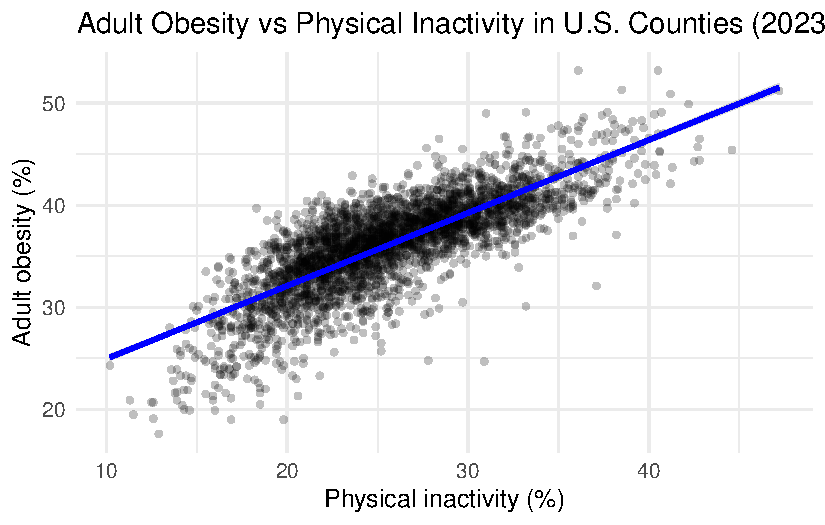
\includegraphics{paper_files/figure-pdf/fig-county-scatter-1.pdf}

}

\caption{\label{fig-county-scatter}Adult Obesity (\%) vs Physical
Inactivity (\%) --- U.S. Counties (2023). Points are counties; the line
is the OLS fit with a 95\% confidence band.}

\end{figure}%

I test the null hypothesis (H\_0:~\beta\_1 = 0) against the two-sided
alternative (H\_1:~\beta\_1 \neq 0). With the estimated slope,
confidence interval, and p-value reported above, there is strong
evidence of a positive association between inactivity and obesity at the
county level.

\begin{longtable}[]{@{}lrrrr@{}}

\caption{\label{tbl-model}Regression results for Adult Obesity on
Physical Inactivity.}

\tabularnewline

\toprule\noalign{}
term & estimate & std.error & statistic & p.value \\
\midrule\noalign{}
\endhead
\bottomrule\noalign{}
\endlastfoot
(Intercept) & 17.811 & 0.256 & 69.568 & 0 \\
inactivity\_pct & 0.714 & 0.010 & 73.051 & 0 \\

\end{longtable}

\FloatBarrier

\section*{References}\label{references}
\addcontentsline{toc}{section}{References}

\phantomsection\label{refs}
\begin{CSLReferences}{1}{0}
\bibitem[\citeproctext]{ref-CHR2023}
County Health Rankings \& Roadmaps. 2023. {``County Health Rankings \&
Roadmaps: 2023 Ranked Measure Data.''}
\url{https://www.countyhealthrankings.org/}.

\bibitem[\citeproctext]{ref-R-base}
R Core Team. 2024. \emph{R: A Language and Environment for Statistical
Computing}. Vienna, Austria: R Foundation for Statistical Computing.
\url{https://www.r-project.org/}.

\bibitem[\citeproctext]{ref-broom}
Robinson, David, Alex Hayes, and Simon Couch. 2024. \emph{Broom: Convert
Statistical Objects into Tidy Tibbles}.
\url{https://broom.tidymodels.org/}.

\bibitem[\citeproctext]{ref-ggplot2-book}
Wickham, Hadley. 2016. \emph{Ggplot2: Elegant Graphics for Data
Analysis}. New York: Springer.

\bibitem[\citeproctext]{ref-ggplot2}
Wickham, Hadley, Winston Chang, Lionel Henry, Thomas Lin Pedersen,
Kohske Takahashi, Claus Wilke, Kara Woo, Hiroaki Yutani, Dewey
Dunnington, and PBC Posit Software. 2024. \emph{Ggplot2: Create Elegant
Data Visualisations Using the Grammar of Graphics}.
\url{https://ggplot2.tidyverse.org/}.

\bibitem[\citeproctext]{ref-dplyr}
Wickham, Hadley, Romain François, Lionel Henry, Kirill Müller, Davis
Vaughan, and PBC Posit Software. 2024. \emph{Dplyr: A Grammar of Data
Manipulation}. \url{https://dplyr.tidyverse.org/}.

\bibitem[\citeproctext]{ref-readr}
Wickham, Hadley, Jim Hester, and posit team. 2024. \emph{Readr: Read
Rectangular Text Data}. \url{https://readr.tidyverse.org/}.

\end{CSLReferences}




\end{document}
